\chapter{Opposing current}
%

% - Purpose & Problem description:
%     These first two parts give reader short details about the test case,
%     the physical phenomena involved and specify how the numerical solution will be validated
%
\section{Purpose}
%
The goal of this test-case is to check the behaviour of \tomawac in presence of
a strong opposing current. When water meets the strong adverse current, with a
velocity that approaches the wave group velocity, waves are blocked. Without
any option for strong current, the amplitud of waves is overestimated.

%
\section{Description of the problem}
%
We present here the simulation of the test case of Lai \cite{Lai1989}. We
present two different options that prevent from overestimation.

Option 1: consider an equilibrium range spectrum (in the presence of ambient
flow) applied as an upper limit for the spectrum Hedges et al
(\cite{Hedges1985})

Option 2: add a dissipative term on the right-hand side of the action balance
equation \cite{Westhuys2012}

For more details on formulations, one can refer to \tomawac documentation,
paragraphs 4.2.3.8.1 and 4.2.3.8.2.

%
\section{Reference}
%
The flume experiment of Lai et al \cite{Lai1989} investigates the
transformation of the wave spectrum on a strong negative current gradient in a
flume of 8~m length and 0.75~m depth. An opposing current flow is induced
along the flume according to figure \ref{courant}
\begin{figure} [!h]
\centering
\includegraphicsmaybe{[width=0.85\textwidth]}{../img/currentx.png}
 \caption{Current of the test case.}
\label{courant}
\end{figure}

\section{Physical parameters}
Concerning the modelling of the opposing current with the first option the
Phillips’s constant in the Pierson-Moskowitz spectrum is equal to 0.0081.
For the second option of this modelling, the dissipation coefficient is equal
to 0.65, and saturation threshold value is taken to $1.75 10^{-3}$.

The white-capping dissipation is the model of Westhuysen 2008. Non linear
transferts between frequencies are calculated by the DIA method.

%
% - Geometry and Mesh:
%     This part describes the mesh used in the computation
%
%
\section{Geometry and Mesh}
%
The bathymetry is as described on figure \ref{bathyop}.
\begin{figure} [!h]
\centering
\includegraphicsmaybe{[width=0.85\textwidth]}{../img/section1d2.png}
 \caption{Bathymetry of the test case.}
\label{bathyop}
\end{figure}

The mesh is made of 1701 nodes and 3200 triangles  and is shown Figure
\ref{mailop}.
\begin{figure} [!h]
\centering
\includegraphicsmaybe{[width=0.85\textwidth]}{../img/mesh.png}
 \caption{Mesh of the domain.}
\label{mailop}
\end{figure}




% - Initial and boundary conditions:
%     This part details both initial and boundary conditions used to simulate the case
%
%
\section{Initial and Boundary Conditions}
%
For both conditions, we take a Jonswap spectrum with a 1.9 cm significant wave
heigth, a peak frequency of 2.2. The angular distribution function follows a
$\cos^{2s} \theta$ distribution with an angular spreading of 65 and a mean
direction of 90.
% - Numerical parameters:
%     This part is used to specify the numerical parameters used
%     (adaptive time step, mass-lumping when necessary...)
%
%
\section{Numerical parameters}
%
Time duration is 400~s, time step is equal to 0.1~s, the spectro-angular mesh
has 72 angles and 36 frequences spread on a geometric progression common ratio
1.1 with a minimum of 0.25.

The option for wave growth limiter is following the Hersbach et Janssen (1999)
parameterisation.

% - Results:
%     We comment in this part the numerical results against the reference ones,
%     giving understanding keys and making assumptions when necessary.
%
%
\section{Results}
%
We show the results obtained Figure \ref{reswaveblocking}. The two options are
efficient to reduce the wave heigth overestimation and lead to a solution
closer to measurements. This shows the interest of including these options in
the case of a strong opposing current.

\begin{figure} [!h]
\centering
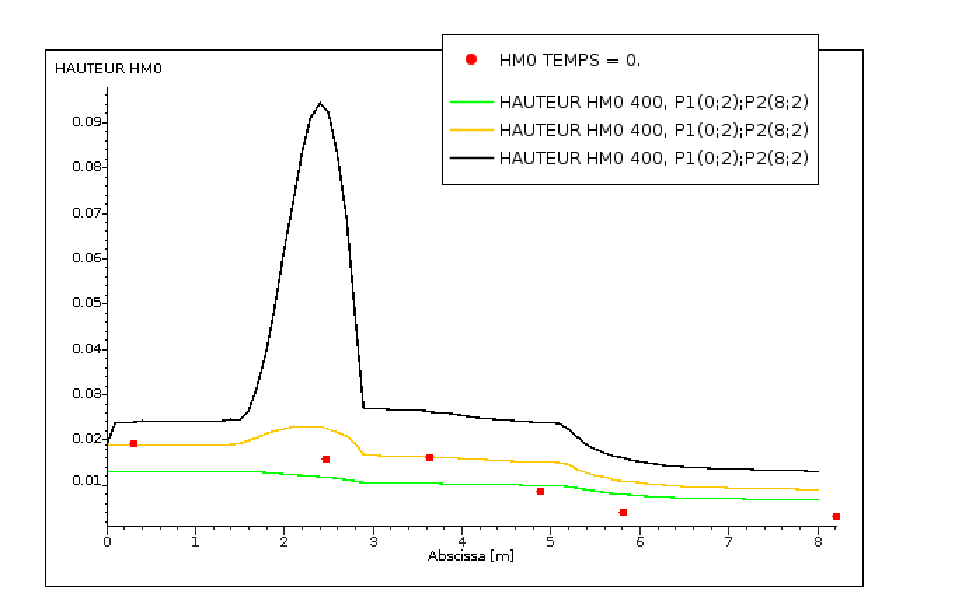
\includegraphics[width=0.85\textwidth]{hauteur.png}
 \caption{Heigth comparison without wave blocking and with the two options.}
\label{reswaveblocking}
\end{figure}

\begin{figure} [!h]
\centering
\includegraphicsmaybe{[width=0.85\textwidth]}{../img/section1d.png}
 \caption{Heigth comparison with the two options for the last validation.}
\label{reswaveblocking2}
\end{figure}

